\documentclass{article}

%\usepackage{amsmath}
\usepackage{amsmath,amsfonts,amssymb,amsthm}
\usepackage{graphicx}
%\graphicspath{{fig/}}


\title{Number of required beds}
\author{Req 550 Syria Team}

\begin{document}

\maketitle 

\section{Approach}

I am using only the simulated maximum of hospitalised. The reasons to restrict
to it are:
\begin{itemize}
    \item The maximum number of required beds corresponds to the peak.
    \item Peaks for different age groups happen at different times, but the
variation is small. Therefore I assume the worst case of all peaks happening at
the same time. This may lead to a slight overestimate on the required number of
beds.
    \item The time series would provide data on the flow of individuals in and
out of the hospital beds. As a consequence of using a mean-field model, the
flow out is proportional to the number of hospitalised individuals. If this has
some effect in the number of available beds, it would be of the order of the
rate of discharges per day, roughly 10\% error (more precisely, order of one
over length of stay in hospital).
    \item The main source of error when estimating the beds requirements in the
region is the lack of knowledge about concurrent outbreaks in different camps.
\end{itemize}
Note that comparing the simulations for camps with 500, 1000 and 2000 people,
the maximum number of hospitalized is proportional to the camp size. I will
scale the results accordingly for the rest of the camps, using the closest
simulation (e.g. for a camp with 345 people, I scale the simulations for 500
people with a factor of $345/500$).

\section{Results}
Using the data in
https://drive.google.com/open?id=1fyrafAu1ikxnELFf8jUw8UHtIDVZtYtJ, the largest
camp in the region has 9219, and the simulations predict that an outbreak in
the camp will require about 183 beds. Figure \ref{fig:beds} shows a boxplot of
the required number of beds for an outbreak in each of the camps. Note that
here the mean is not relevant: an outbreak in the largest camp will require at
least 183, and any other concurrent outbreak will increase that number. The
Figure is included to show what the majority of camps would require for
independent outbreaks.

\begin{figure}[ht]
    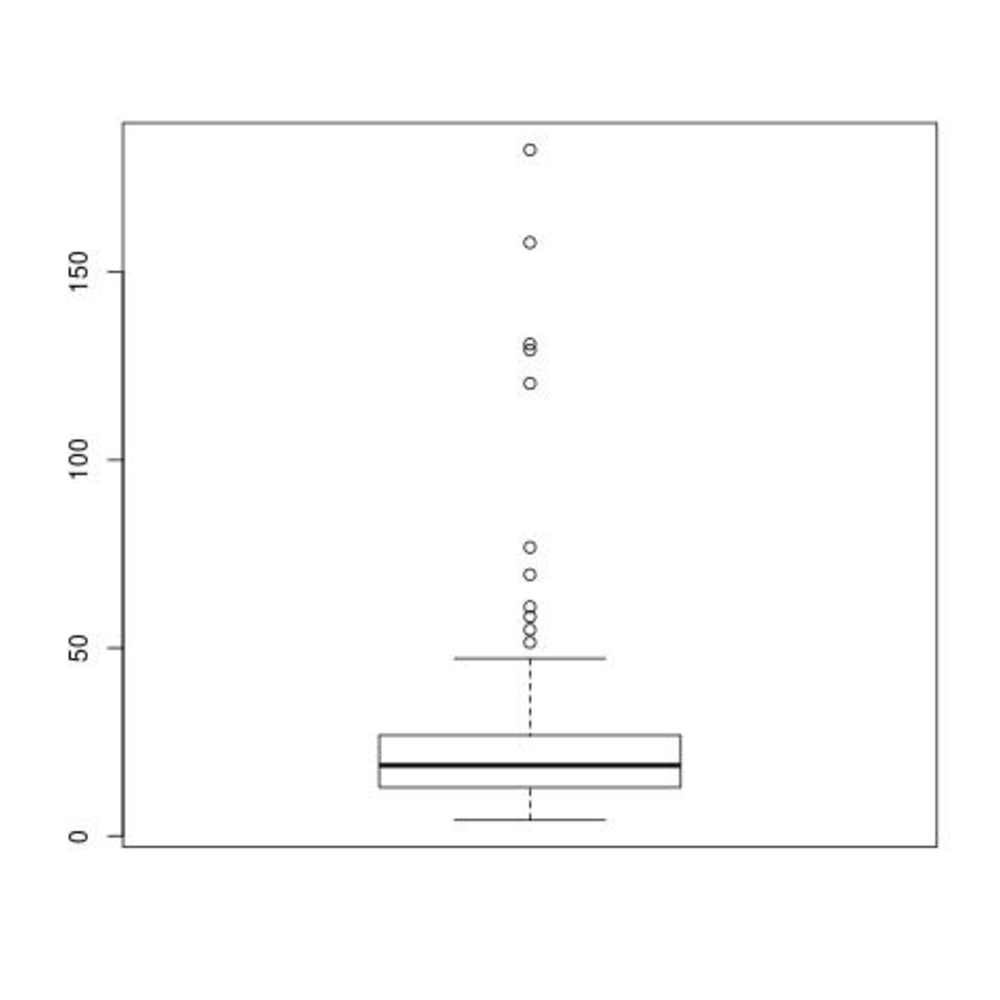
\includegraphics[width=.95\linewidth]{beds_box}
    \caption{Number of beds required in different camps. Note that each data
point is an independent outbreak; concurrent outbreaks (i.e. outbreaks
happening at the same time in different camps) would require many more beds
available.}\label{fig:beds}
\end{figure}


\end{document}
